\documentclass{article}
\usepackage[utf8]{inputenc}
\usepackage{enumitem}
\usepackage{amsmath}
\usepackage{algorithm}
\usepackage[noend]{algpseudocode}
\usepackage[margin=1.25in]{geometry}
\usepackage{pdfpages}

\usepackage{listings}
\usepackage{color}
\usepackage{graphicx}


\definecolor{codegreen}{rgb}{0,0.6,0}
\definecolor{codegray}{rgb}{0.5,0.5,0.5}
\definecolor{codepurple}{rgb}{0.58,0,0.82}
\definecolor{backcolour}{rgb}{0.95,0.95,0.92}
 
\lstdefinestyle{mystyle}{
    backgroundcolor=\color{backcolour},   
    commentstyle=\color{codegreen},
    keywordstyle=\color{magenta},
    numberstyle=\tiny\color{codegray},
    stringstyle=\color{codepurple},
    basicstyle=\footnotesize,
    breakatwhitespace=false,         
    breaklines=true,                 
    captionpos=b,                    
    keepspaces=true,                 
    numbers=left,                    
    numbersep=5pt,                  
    showspaces=false,                
    showstringspaces=false,
    showtabs=false,                  
    tabsize=2
}

\lstset{
  tabsize=4,
  language=c++,
  style = mystyle
}

\title{CS352 (Winter 2018) - Homework 6}
\author{Marc Tibbs (tibbsm@oregonstate.edu)}
\date{Due Date: February 25, 2018}

\begin{document}

\maketitle

\noindent \textbf{Problem 1:} \textit{(7 points)} Shortest paths can be cast as an LP using distances dv from the source s to a particular vertex v as variables.\\

\noindent \textbf{We can compute the shortest path from s to t in a weighted directed graph by solving.}\\
max dt \\
subject to\\
\indent ds = 0\\
\indent dv – du $\leq$ w(u,v) for all (u,v)$\in$E
\\[.25cm]

\noindent \textbf{We can compute the single-source by changing the objective function to}\\
max $\sum_{v\in V} dv$
\\[.25cm]

\noindent Use linear programming to answer the questions below. Submit a copy of the LP code and output.
\\[.25cm]

\noindent \textbf{a) Find the distance of the shortest path from G to C in the graph below.}\\
The shortest path is G, H, B, C with a distance of 16. A copy of the LP code and output is in the appendix.
\\[.25cm]

\noindent \textbf{b) Find the distances of the shortest paths from G to all other vertices.}\\
A copy of the LP code and output is in the appendix.
\\[.25cm]
\begin{center}
 \begin{tabular}{|| c | c ||} 
 \hline
 Vertex & Distance from G to Vertex\\ 
 \hline\hline
 a & 7 \\ 
 \hline
 b & 12 \\
 \hline
 c & 16 \\
 \hline
 d & 2 \\
 \hline
 e & 19 \\
 \hline
 f & 17 \\
 \hline
 g & 0 \\
 \hline
 h & 3 \\
 \hline
\end{tabular}
\end{center}

\newpage

\noindent \textbf{Problem 2:} \textit{(7 points)} Acme Industries produces four types of men’s ties using three types of material. Your job is to determine how many of each type of tie to make each month. The goal is to maximize profit, profit per tie = selling price - labor cost – material cost. Labor cost is \$0.75 per tie for all four types of ties. The material requirements and costs are given below.\\

\begin{flushleft}
 \begin{tabular}{|| l | l | l ||}
 \hline
 Material & Cost / Yard & Yards / Month\\ 
 \hline\hline
 Silk & \$20 & 1,000 \\ 
 \hline
 Polyester & \$6 & 2,000 \\
 \hline
 Cotton & \$9 & 1,250 \\
 \hline
\end{tabular}
\end{flushleft}

\begin{flushleft}
 \begin{tabular}{|| l | l | l | l | l ||} 
 \hline
 Product Info & Silk(s) & Poly(p) & Blend 1(b)& Blend2(c)\\ 
 \hline\hline
 Sale Price & \$6.70 & \$3.55 & \$4.31 & \$4.81  \\ 
 \hline
 Min. Units / Month & 6,000 & 10,000 & 13,000 & 6,000 \\
 \hline
 Max. Units / Month & 7,000 & 14,000 & 16,000 & 8,500 \\
 \hline
 \end{tabular}
\end{flushleft}

\begin{flushleft}
 \begin{tabular}{|| l | l | l | l | l ||} 
 \hline
  Material Info & Silk(s) & Poly(p) & Blend 1(b)& Blend2(c)\\ 
 \hline\hline
 Silk & 0.125 & 0 & 0 & 0  \\ 
 \hline
 Polyester & 0 & 0.08 & 0.05 & 0.03 \\
 \hline
 Cotton & 0 & 0 & 0.05 & 0.07 \\
 \hline
 \end{tabular}
\end{flushleft}


\begin{flushleft}
 \begin{tabular}{|| l | l | l | l | l ||} 
 \hline
  Type & Selling Price & Labor & Material & Profit/Tie\\ 
 \hline\hline
 Silk(s) & 6.7 & 0.75 & 2.5 & 3.45  \\ 
 \hline
 Polyester(p) & 3.55 & 0.75 & 0.48 & 2.32 \\
 \hline
 Blend 1(b) & 4.31 & 0.75 & 0.75 & 2.81 \\
 \hline
 Blend 2(c) & 4.81 & 0.75 & 0.81 & 3.25 \\
 \hline
 \end{tabular}
\end{flushleft}

\noindent Formulate the problem as a linear program with an objective function and all constraints. Determine the optimal solution for the linear program using any software you want. What are the optimal numbers of ties of each type to maximize profit? Include a copy of the code and output.\\[.25cm]

\textbf{The maximized profit is \$120,196, which you would get from selling 7,000 silk, 13,625 polyester, 13,100 blend1, and 8,500 blend2 ties. A copy of the LP code and output is in the appendix.}
\\[.25cm]

\newpage

\noindent \textbf{Problem 3: Transshipment Model} \textit{(7 points)}\\ This is an extension of the transportation model. There are now intermediate transshipment points added between the sources (plants) and destinations (retailers). Items being shipped from a Plant ($p_i$) must be shipped to a Warehouse ($w_j$) before being shipped to the Retailer ($r_k$). Each Plant will have an associated supply ($s_i$) and each Retailer will have a demand ($d_k$). The number of plants is n, number of warehouses is q and the number of retailers is m. The edges (i,j) from plant ($p_i$)to warehouse ($w_j$) have costs associated denoted cp(i,j). The edges (j,k) from a warehouse ($w_j$)to a retailer ($r_k$) have costs associated denoted cw(j,k).
\\[.25cm]

The graph below shows the transshipment map for a manufacturer of refrigerators. Refrigerators are produced at four plants and then shipped to a warehouse (weekly) before going to the retailer.
\\[.25cm]

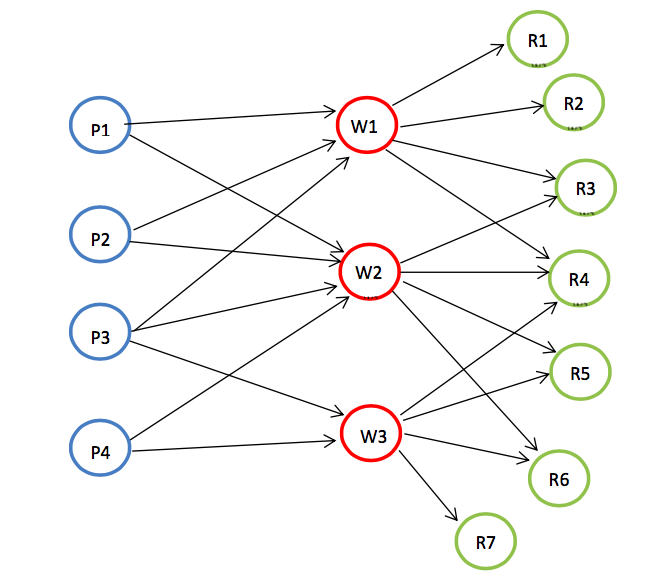
\includegraphics[scale=.5]{TRANS}\\

Below are the costs of shipping from a plant to a warehouse and then a warehouse to a retailer. If it is impossible to ship between the two locations an X is placed in the table.\\

\begin{flushleft}
 \begin{tabular}{|| l | l | l | l ||}
 \hline
 Cost & W1 & W2 & W3\\ 
 \hline\hline
 P1 & \$10 & \$15 & X\\ 
 \hline
 P2 & \$11 & \$8 & X\\ 
 \hline
 P3 & \$13 & \$8 & \$9\\  
 \hline
 P4 & X & \$14 & \$8\\  
 \hline
\end{tabular}
\end{flushleft}

\begin{flushleft}
 \begin{tabular}{|| l | l | l | l | l | l | l  | l ||}
 \hline
 Cost & R1 & R2 & R3 & R4 & R5 & R6 & R7\\ 
 \hline\hline
 W1 & \$5 & \$6 & \$7 & \$10 & X & X & X\\ 
 \hline
 W2 & X & X & \$12 & \$8 & \$10 & \$14 & X\\ 
 \hline
 W3 & X & X & X & \$14 & \$12 & \$12 & \$6\\ 
 \hline
\end{tabular}
\end{flushleft}

\noindent The tables below give the capacity of each plant (supply) and the demand for each retailer (per week).

\begin{flushleft}
 \begin{tabular}{|| l | l | l | l | l ||}
 \hline
  & P1 & P2 & P3 & P4\\ 
 \hline\hline
 Supply & 150 & 450 & 250 & 150\\ 
 \hline
\end{tabular}
\end{flushleft}

\begin{flushleft}
 \begin{tabular}{|| l | l | l | l | l | l | l | l ||}
 \hline
 & R1 & R2 & R3 & R4 & R5 & R6 & R7\\ 
 \hline\hline
 Demand & 100 & 150 & 100 & 200 & 200 & 150 & 100\\ 
 \hline
\end{tabular}
\end{flushleft}

\noindent Your goal is to determine the number of refrigerators to be shipped plants to warehouses and then warehouses to retailers to minimize the cost. Formulate the problem as a linear program with an objective function and all constraints. Determine the optimal solution for the linear program using any software you want. What are the optimal shipping routes and minimum cost.\\
Include a copy of the code and output.
\\[.25cm]
\textbf{The minimum cost is \$17,100. The optimal shipping routes are shown in the graph below. A copy of the LP code and output is in the appendix.}

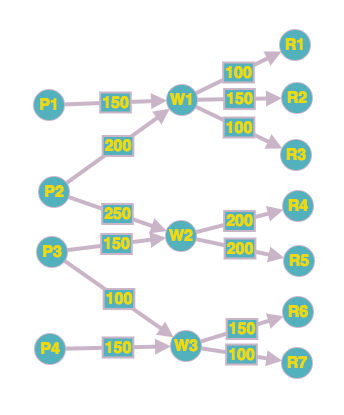
\includegraphics[scale=.5]{TRANS1}\\

\newpage

\noindent \textbf{Problem 4: A Mixture Problem} \textit{(9 points)}\\ 
Veronica the owner of Very Veggie Vegeria is creating a new healthy salad that is low in calories but meets certain nutritional requirements. A salad is any combination of the following ingredients:\\
\indent Tomato, Lettuce, Spinach, Carrot, Smoked Tofu, Sunflower Seeds, Chickpeas, Oil
\\
Each salad must contain:
\begin{itemize}
    \item At least 15 grams of protein
    \item At least 2 and at most 8 grams of fat
    \item At least 4 grams of carbohydrates
    \item At most 200 milligrams of sodium
    \item At least 40\% leafy greens by mass.
\end{itemize}

The nutritional contents of these ingredients (per 100 grams) and cost are:

\begin{flushleft}
 \begin{tabular}{|| l | l | l | l | l | l | l ||}
 \hline
 Ingredient & Calories & Protein(g) & Fat(g) & Carbs(g) & Sodium(mg) & Cost(100g)\\ 
 \hline\hline
 Tomato & 21 & 0.85 & 0.33 & 4.64 & 9 & \$1.00 \\ 
 \hline
 Lettuce & 16 & 1.62 & 0.20 & 2.37 & 28 & \$0.75 \\ 
 \hline
 Spinach & 40 & 2.86 & 0.39 & 3.63 & 65 & \$0.50 \\ 
 \hline
 Carrot & 41 & 0.93 & 0.24 & 9.58 & 69 & \$0.50 \\ 
 \hline
 Sunflower Seeds & 585 & 23.4 & 48.7 & 15 & 3.8 & \$0.45 \\ 
 \hline
 Smoked Tofu & 120 & 16 & 5 & 3 & 120 & \$2.15 \\ 
 \hline
 Chickpeas & 164 & 9 & 2.6 & 27 & 78 & \$0.95 \\ 
 \hline
 Oil & 884 & 0 & 100 & 0 & 0 & \$2.00 \\ 
 \hline
\end{tabular}
\end{flushleft}

\noindent \textbf{Part A: }Determine the combination of ingredients that minimizes calories but meets all nutritional requirements. Formulate the problem as a linear program with an objective function and all constraints. Determine the optimal solution for the linear program using any software you want. What is the cost of the low calorie salad?
\\[.25cm]
\textbf{The low calorie salad is made up of steamed tofu and lettuce. It costs \$2.33.}
\begin{flushleft}
 \begin{tabular}{|| l | l | l | l | l | l | l ||}
 \hline
 Ingredient & Calories & Protein(g) & Fat(g) & Carbs(g) & Sodium(mg) & Cost(100g)\\ 
 \hline\hline
 Lettuce (58.5 grams) & 9.4 & 0.9 & 0.1 & 1.4 & 16.4 & \$0.44 \\ 
 \hline
 Smoked Tofu (87.8 grams) & 105.4 & 14.1 & 4.4 & 2.6 & 105.4 & \$1.89 \\ 
 \hline
 Total (146.3 grams) & 114.8 & 15 & 4.5 & 4 & 121.8 & \$2.33 \\ 
 \hline
\end{tabular}
\end{flushleft}

\noindent \textbf{Part B: }Part B: Veronica realizes that it is also important to minimize the cost associated with the new salad. Unfortunately some of the ingredients can be expensive. Determine the combination of ingredients that minimizes cost. Formulate the problem as a linear program with an objective function and all constraints. Determine the optimal solution for the linear program using any software you want. How many calories are in the low cost salad?
\\[.25cm]
\textbf{The low cost salad is made up of chickpeas, sunflower seeds, and spinach. It has 278 calories. A copy of the LP code and output is in the appendix.}
\begin{flushleft}
 \begin{tabular}{|| l | l | l | l | l | l | l ||}
 \hline
 Ingredient & Calories & Protein(g) & Fat(g) & Carbs(g) & Sodium(mg) & Cost(100g)\\ 
 \hline\hline
 Spinach (83.2 grams) & 33.3 & 2.4 & 0.3 & 3 & 54.1 & \$0.42 \\ 
 \hline
 Sunflower Seeds (9.6 grams) & 56.2 & 2.2 & 4.7 & 1.4 & 0.4 & \$0.04 \\ 
 \hline 
 Chickpeas (115.2 grams) & 189 & 10.4 & 3 & 31.1 & 89.9 & \$1.09 \\ 
 \hline
 Total (208 grams) & 278.5 & 15 & 8 & 35.5 & 144.4 & \$1.55 \\ 
 \hline
\end{tabular}
\end{flushleft}



\newpage

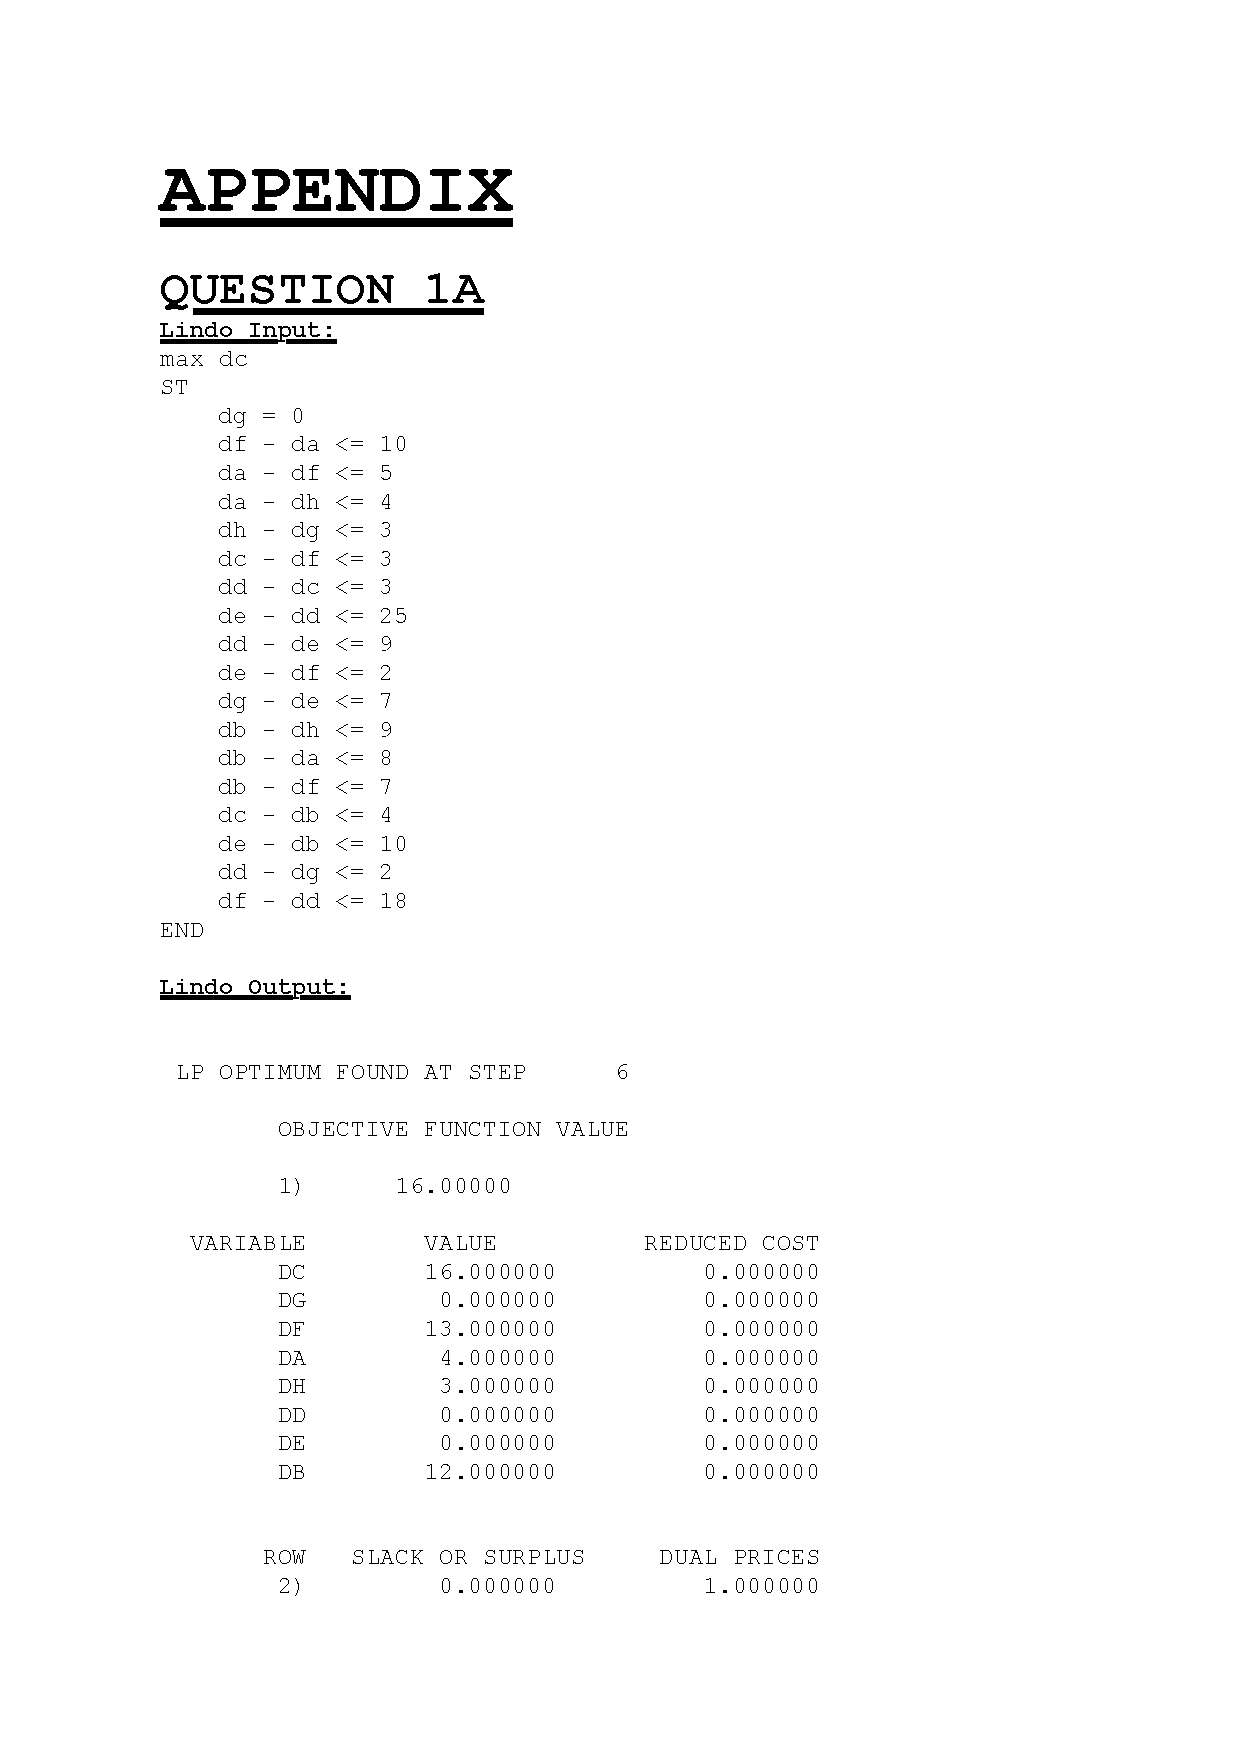
\includepdf[pages=-]{LINDO.pdf}


\end{document}
